% В этом файле следует писать текст работы, разбивая его на
% разделы (section), подразделы (subsection) и, если нужно,
% главы (chapter).

% Предварительно следует указать необходимую информацию
% в файле SETUP.tex

%% В этот файл не предполагается вносить изменения

% В этом файле следует указать информацию о себе
% и выполняемой работе.

\documentclass [fontsize=14pt, paper=a4, pagesize, DIV=calc]%
{scrreprt}
% ВНИМАНИЕ! Для использования глав поменять
% scrartcl на scrreprt

% Здесь ничего не менять
\usepackage [T2A] {fontenc}   % Кириллица в PDF файле
\usepackage [utf8] {inputenc} % Кодировка текста: utf-8
\usepackage [russian] {babel} % Переносы, лигатуры

%%%%%%%%%%%%%%%%%%%%%%%%%%%%%%%%%%%%%%%%%%%%%%%%%%%%%%%%%%%%%%%%%%%%%%%%
% Создание макроса управления элементами, специфичными
% для вида работы (курс., бак., маг.)
% Здесь ничего не менять:
\usepackage{ifthen}
\newcounter{worktype}
\newcommand{\typeOfWork}[1]
{
	\setcounter{worktype}{#1}
}

% ВНИМАНИЕ!
% Укажите тип работы: 0 - курсовая, 1 - бак., 2 - маг.,
% 3 - бакалаврская с главами.
\typeOfWork{2}
% Считается, что курсовая и бак. бьются на разделы (section) и
% подразделы (subsection), а маг. — на главы (chapter), разделы и
%  подразделы. Если хочется,
% чтобы бак. была с главами (например, если она большая),
% надо выбрать опцию 3.

% Если при выборе 2 или 3 вы забудете поменять класс
% документа на scrreprt (см. выше, в самом начале),
% то получите ошибку:
% ./aux/appearance.tex:52: Package scrbase Error: unknown option ` chapterprefix=

%%%%%%%%%%%%%%%%%%%%%%%%%%%%%%%%%%%%%%%%%%%%%%%%%%%%%%%%%%%%%%%%%%%%%%%%
% Информация об авторе и работе для титульной страницы

\usepackage {titling}

% Имя автора в именительном падеже (для маг.)
\newcommand {\me}{%
А.\,А.~Мухаррам
}

% Имя автора в родительном падеже (для курсовой и бак.)
\newcommand {\byme}{%
А.\,А.~Мухаррам
}

% Любимый научный руководитель
\newcommand{\supervisor}%
{ст. преп. В. Н. Брагилевский}

% идентифицируем пол (только для курсовой и бак.)
\newcommand{\bystudent}{
студента %студентки % Для курсовой: с большой буквы
}

% Год публикации
\date{2017}

% Название работы
\title{Равносильность TMS отношения и отношения уточнения абстрактной транзакционной памяти конкретной}

% Кафедра
%
\newboolean{needchair}
\setboolean{needchair}{false} % на ФИИТ не пишется (false), на ПМИ есть (true)

\newcommand {\thechair} {%
Кафедра компьютерного и аналогового моделирования светлого будущего%
}

\newcommand {\direction} {%
Направление подготовки\\
Фундаментальная информатика и информационные технологии%
}% Прикладная математика и информатика

%%%%%%%%%%%%%%%%%%%%%%%%%%%%%%%%%%%%%%%%%%%%%%%%%%%%%%%%%%%%%%%%%%%%%%%%
% Другие настраиваемые элементы текста

% Листинги с исходным кодом программ: укажите язык программирования
\usepackage{listings}
\lstset{
    language=[ISO]C++,%  Язык указать здесь
    basicstyle=\small\ttfamily,
    breaklines=true,%
    showstringspaces=false%
    inputencoding=utf8x%
}
% полный список языков, поддерживаемых данным пакетом, есть,
% например, здесь (стр. 13):
% ftp://ftp.tex.ac.uk/tex-archive/macros/latex/contrib/listings/listings.pdf

% Гиперссылки: настройте внешний вид ссылок
\usepackage%
[pdftex,unicode,pdfborder=0,draft=false,%backref=page,
    hidelinks, % убрать, если хочется видеть ссылки: это
               % удобно в PDF файле, но не должно появиться на печати
    bookmarks=true,bookmarksnumbered=false,bookmarksopen=false]%
{hyperref}


\usepackage {amsmath}      % Больше математики
\usepackage {amssymb}
\usepackage {textcase}     % Преобразование к верхнему регистру
\usepackage {indentfirst}  % Красная строка первого абзаца в разделе

\usepackage {fancyvrb}     % Листинги: определяем своё окружение Verb
\DefineVerbatimEnvironment% с уменьшенным шрифтом
	{Verb}{Verbatim}
	{fontsize=\small}

% Вставка рисунков
\usepackage {graphicx}

% Общее оформление
% ----------------------------------------------------------------
% Настройка внешнего вида

%%% Шрифты

% если закомментировать всё — консервативная гарнитура Computer Modern
\usepackage{paratype} % профессиональные свободные шрифты
%\usepackage {droid}  % неплохие свободные шрифты от Google
%\usepackage{mathptmx}
%\usepackage {mmasym}
%\usepackage {psfonts}
%\usepackage{lmodern}
%var1: lh additions for bold concrete fonts
%\usepackage{lh-t2axccr}
%var2: the package below could be covered with fd-files
%\usepackage{lh-t2accr}
%\usepackage {pscyr}

% Геометрия текста

\usepackage{setspace}       % Межстрочный интервал
\onehalfspacing

\newlength\MyIndent
\setlength\MyIndent{1.25cm}
\setlength{\parindent}{\MyIndent} % Абзацный отступ
\frenchspacing            % Отключение лишних отступов после точек
\KOMAoptions{%
    DIV=calc,         % Пересчёт геометрии
    numbers=endperiod % точки после номеров разделов
}

                            % Консервативный вариант:
%\usepackage                % ручное задание геометрии
%[%                         % (не рекомендуется в проф. типографии)
%  margin = 2.5cm,
  %includefoot,
  %footskip = 1cm
%] %
%  {geometry}

%%% Заголовки



\ifthenelse{\equal{\theworktype}{2}}{%
\KOMAoptions{%
    numbers=endperiod,% точки после номеров разделов
    headings=normal,   % размеры заголовков поменьше стандартных
    chapterprefix=true,% Печатать слово Глава в магистерской
    appendixprefix=true% Печатать слово Приложение
}
}

% шрифт для оформления глав и названия содержания
\newcommand{\SuperFont}{\Large\sffamily\bfseries}

% Заголовок главы
\ifthenelse{\value{worktype} > 1}{%
\renewcommand{\SuperFont}{\Large\normalfont\sffamily}
\newcommand{\CentSuperFont}{\centering\SuperFont}
\usepackage{fncychap}
\ChNameVar{\SuperFont}
\ChNumVar{\CentSuperFont}
\ChTitleVar{\CentSuperFont}
\ChNameUpperCase
\ChTitleUpperCase
}

% Заголовок (под)раздела с абзацного отступа
\addtokomafont{sectioning}{\hspace{\MyIndent}}

\renewcommand*{\captionformat}{~---~}
\renewcommand*{\figureformat}{Рисунок~\thefigure}

%%% Оглавление
\usepackage{tocloft}

% шрифт и положение заголовка
\ifthenelse{\value{worktype} > 1}{%
\renewcommand{\cfttoctitlefont}{\hfil\SuperFont\MakeUppercase}
}{
\renewcommand{\cfttoctitlefont}{\hfil\SuperFont}
}

% слово Глава
\usepackage{calc}
\ifthenelse{\value{worktype} > 1}{%
\renewcommand{\cftchappresnum}{Глава }
\addtolength{\cftchapnumwidth}{\widthof{Глава }}
}

% Очищаем оформление названий старших элементов в оглавлении
\ifthenelse{\value{worktype} > 1}{%
\renewcommand{\cftchapfont}{}
\renewcommand{\cftchappagefont}{}
}{
\renewcommand{\cftsecfont}{}
\renewcommand{\cftsecpagefont}{}
}

\ifthenelse{\value{worktype} > 1}{%
    \renewcommand{\cftchapaftersnum}{.}
}{
\renewcommand{\cftsecaftersnum}{.}
\renewcommand{\cftsubsecaftersnum}{.}
}
%%% Списки (enumitem)

\usepackage {enumitem}      % Списки с настройкой отступов
\setlist %
{ %
  leftmargin = \parindent, itemsep=.5ex, topsep=.4ex
} %

% По ГОСТу нумерация должны быть буквами: а, б...
%\makeatletter
%    \AddEnumerateCounter{\asbuk}{\@asbuk}{м)}
%\makeatother
%\renewcommand{\labelenumi}{\asbuk{enumi})}
%\renewcommand{\labelenumii}{\arabic{enumii})}

%%% Таблицы: выбрать более подходящие

\usepackage{booktabs} % считаются наиболее профессионально выполненными
%\usepackage{ltablex}
%\newcolumntype {L} {>{---}l}

%%% Библиография

\usepackage{csquotes}        % Оформление списка литературы
\usepackage[
  backend=biber,
  hyperref=auto,
  language=auto,
  citestyle=gost-numeric,
  bibstyle=gost-numeric,
]{biblatex}
\addbibresource{biblio.bib} % Файл с лит.источниками

% Настройка величины отступа в списке
\ifthenelse{\value{worktype} < 2}{%
\defbibenvironment{bibliography}
  {\list
     {\printtext[labelnumberwidth]{%
    \printfield{prefixnumber}%
    \printfield{labelnumber}}}
     {\setlength{\labelwidth}{\labelnumberwidth}%
      \setlength{\leftmargin}{\labelwidth}%
      \setlength{\labelsep}{\dimexpr\MyIndent-\labelwidth\relax}% <----- default is \biblabelsep
      \addtolength{\leftmargin}{\labelsep}%
      \setlength{\itemsep}{\bibitemsep}%
      \setlength{\parsep}{\bibparsep}}%
      \renewcommand*{\makelabel}[1]{\hss##1}}
  {\endlist}
  {\item}
}{}

% ----------------------------------------------------------------
% Настройка переносов и разрывов страниц

\binoppenalty = 10000      % Запрет переносов строк в формулах
\relpenalty = 10000        %

\sloppy                    % Не выходить за границы бокса
%\tolerance = 400          % или более точно
\clubpenalty = 10000       % Запрет разрывов страниц после первой
\widowpenalty = 10000      % и перед предпоследней строкой абзаца

% ----------------------------


% Стили для окружений типа Определение, Теорема...
% Оформление теорем (ntheorem)

\usepackage [thmmarks, amsmath] {ntheorem}
\theorempreskipamount 0.6cm

\theoremstyle {plain} %
\theoremheaderfont {\normalfont \bfseries} %
\theorembodyfont {\slshape} %
% \theoremsymbol {\ensuremath {_\Box}} %
\theoremseparator {:} %
\newtheorem {mystatement} {Утверждение} [section] %
\newtheorem {mylemma} {Лемма} [section] %
\newtheorem {mycorollary} {Следствие} [section] %
\newtheorem{theorem}{Теорема}
\newtheorem{lemma}{Лемма}

\theoremstyle {plain} %
\theoremseparator {.} %
\theoremsymbol {\ensuremath {_\diamondsuit}} %
\newtheorem {mydefinition} {Определение} %

\theoremstyle {plain} %
\theoremheaderfont {\normalfont \bfseries} 
\theorembodyfont {\normalfont} 
%\theoremsymbol {\ensuremath {_\Box}} %
\theoremseparator {.} %
\newtheorem {mytask} {Задача} [section]%
\renewcommand{\themytask}{\arabic{mytask}}

\theoremheaderfont {\normalfont \bfseries}
% \theoremheaderfont {\scshape} %
\theorembodyfont {\upshape} %
\theoremstyle {nonumberplain} %
\theoremseparator {:} %
\theoremsymbol {\rule {1ex} {1ex}} %
\newtheorem {myproof} {Доказательство} %

\theorembodyfont {\upshape} %
%\theoremindent 0.5cm
\theoremstyle {nonumberbreak} \theoremseparator {\\} %
\theoremsymbol {\ensuremath {\ast}} %
\newtheorem {myexample} {Пример} %
\newtheorem {myexamples} {Примеры} %

\theoremheaderfont {\itshape} %
\theorembodyfont {\upshape} %
\theoremstyle {nonumberplain} %
\theoremseparator {:} %
\theoremsymbol {\ensuremath {_\triangle}} %
\newtheorem {myremark} {Замечание} %
\theoremstyle {nonumberbreak} %
\newtheorem {myremarks} {Замечания} %


% Титульный лист
% Макросы настройки титульной страницы
% В этот файл не предполагается вносить изменения

%\usepackage {showframe}

% Вертикальные отступы на титульной странице
\newcommand{\vgap}{\vspace{10pt}}

% Помещение города и даты в нижний колонтитул
\usepackage{scrlayer}
\DeclareNewLayer[
  foot,
  foreground,
  contents={%
    \raisebox{\dp\strutbox}[\layerheight][0pt]{%
      \parbox[b]{\layerwidth}{\centering Ростов-на-Дону\\ \thedate%
       \\\mbox{}
       }}%
  }
]{titlepage.foot.fg}
\DeclareNewPageStyleByLayers{titlepage}{titlepage.foot.fg}


\AtBeginDocument %
{ %
  %
  \begin{titlepage}
  %
    \thispagestyle{titlepage}

    {\centering
    %
    \MakeTextUppercase {МИНИСТЕРСТВО ОБРАЗОВАНИЯ И НАУКИ РФ}

    \vgap

    Федеральное государственное автономное образовательное\\
    учреждение высшего образования\\
    \MakeTextUppercase {Южный федеральный университет}

    \vgap

  Институт математики, механики и компьютерных наук
    им.~И.\,И.~Воровича

    \vgap

    \direction

    \ifthenelse{\boolean{needchair}}{
    \vgap

    \thechair}{}

    \vspace* {\fill}

    \ifthenelse{\value{worktype} = 2}{%
    \me

    \vgap}{}

    \MakeTextUppercase{\thetitle}

    \ifthenelse{\value{worktype} = 2}{%
     \vgap

    Магистерская диссертация}{}
    \ifthenelse{\value{worktype} = 0}{
     \vgap

    Курсовая работа
    }{}%

    \vspace {\fill}

    \begin{flushright}
    \ifthenelse{\value{worktype} = 1 \OR \value{worktype} = 3}{
    Выпускная квалификационная работа\\
    на степень бакалавра%
   }{}%
    \ifthenelse{\value{worktype} = 1 \OR \value{worktype} = 0 \OR \value{worktype} = 3}{%
    \bystudent\\
    \byme
    }{}

    \vgap

    Научный руководитель:\\
    \supervisor\\
    \ifthenelse{\value{worktype} = 2}{%
    Рецензент:\\
    ученая степень, ученое звание [, должность]
    И. О. Фамилия
    }{}
  \end{flushright}

    \vspace {\fill}

  %Ростов-на-Дону

    %\thedate

  }\end{titlepage}
  %
  %
  \tableofcontents
  %
  \clearpage
} %



% Команды для использования в тексте работы
% макросы для начала введения и заключения
\newcommand{\Intro}{\addsec{Введение}}
\ifthenelse{\value{worktype} > 1}{%
    \renewcommand{\Intro}{\addchap{Введение}}%
}

\newcommand{\Conc}{\addsec{Заключение}}
\ifthenelse{\value{worktype} > 1}{%
    \renewcommand{\Conc}{\addchap{Заключение}}%
}

% Правильные значки для нестрогих неравенств и пустого множества
\renewcommand {\le} {\leqslant}
\renewcommand {\ge} {\geqslant}
\renewcommand {\emptyset} {\varnothing}

% N ажурное: натуральные числа
\newcommand {\N} {\ensuremath{\mathbb N}}

% значок С++ — используйте команду \cpp
\newcommand{\cpp}{C\nolinebreak\hspace{-.05em}%
\raisebox{.2ex}{+}\nolinebreak\hspace{-.10em}%
\raisebox{.2ex}{+}}

% Неразрывный дефис, который допускает перенос внутри слов,
% типа жёлто-синий: нужно писать жёлто"/синий.
\makeatletter
    \defineshorthand[russian]{"/}{\mbox{-}\bbl@allowhyphens}
\makeatother


\endinput

% Конец файла


\begin{document}

\Intro


% Если typeOfWork в SETUP.tex задан как 2 или 3, то начинать
% надо не с section (раздел), а с главы (chapter)
\chapter{Синтаксис и семантика языка программирования}
В данной главе будет приведена семантика и синтаксис языка программирования, описанного в работах ~\cite{tms_article} и ~\cite{opacity_article}. В данный язык введён ряд ограничений. В программе запрещено явно прерывать выполнение транзакций, использовать вложенные атомарные блоки и транзакции. 

\section{Синтаксис}
Рассмотрим язык программирования, в котором программа $P$ представляется в виде параллельной композиции потоков  $C_t,\, t \in ThreadId=\{1, \ldots, m \}$: $P = C_1 \parallel \ldots \parallel C_m$. У каждого потока $t \in Threads$ есть набор локальных переменных $LVar_t = \{x,y, \ldots \}$ и общий набор глобальных переменных $GVar = \{g, \ldots \}$. Все переменные целого типа. Обозначим  $Var = GVar \uplus \biguplus_{t = 1}^m LVar_{t}$ --- множество всех переменных программы. У потоков также есть доступ к транзакционной памяти, которая управляет фиксированным набором объектов $Obj = \{o, \ldots \}$. У каждого объекта есть множество методов, которые могут быть вызваны потоками. Предполагается, что каждый метод принимает на входе целое значение и возвращает в качестве результата целое значение. У всех объектов транзакционной памяти один и тот же набор методов $Method = \{f, \ldots \}$. Синтаксис команд $C$ рассматриваемого языка программирования стандартный. $C$ может иметь вид: $$ c \,|\, C;C \,|\, while \left (b\right) \, do \, C \,|\, if \left (b\right) then \, C\, else \, C \, | \, x := atomic \, \{ C \} \, | \, x := o.f(e), $$ где $b$ и $e$ обозначают логические и целые операции над локальными переменными. Синтаксис включает примитивную команду $c$ из множества $PComm$, последовательность команд, цикл, условный оператор, атомарный блок и вызов методов объектов. Примитивные команды исполняются атомарно. Множество $PComm$ включает присваивания значений локальным и глобальным переменным и специальную операцию fault, которая останавливает исполнение программы в ошибочном состоянии. Следовательно, fault вызывается при некорректных вычислениях, таких как деление на ноль.

Атомарный блок $x := atomic \, \{C\}$ исполняет $C$ как транзакцию, которую транзакционная память может зафиксировать или прервать. Решение системы ($aborted$ или $committed$) будет записано в локальную переменную $x$. 

В данный языке программирования введено ограничение доступа к переменным и объектам транзакционной памяти. Вызов методов объектов транзакционной памяти возможен только внутри транзакций, доступ к глобальным переменным осуществляется только вне транзакций. Локальные переменные доступны в обоих случаях, но потокам запрещен доступ к локальным переменным других потоков.

Для формального описания ограничения доступа примитивных команд к переменным, множество $PComm - \{fault\}$ разделяется на два подмножества: $\biguplus_{t=1}^m (LPcomm_t \uplus GPcomm_t)$. Команды из подмножества $LPcomm_t$ имеют доступ только к локальным переменным потока $t$ ($LVar_t$). У команд из подмножества $GPcomm_t$ есть доступ как к локальным переменным потока $t$, так и к глобальным переменным программы ($LVar_t \uplus GVar$). 

\section{Модель вычисления}
Прежде чем перейти к определению семантики данного языка программирования, введём основные термины. 

\begin{mydefinition}\label{def1} Пусть $ActionId$ --- множество идентификаторов действий. Действие интерфейса $\psi$ транзакционной памяти ($TM$) может иметь одно из следующих представлений:\\

\begin{tabular}{llr}
\hline
Запрос  & Ответ \\
\hline
$(a, t, txbegin)$ & $(a, t, OK)$ & $(a, t, aborted)$     \\
$(a, t, txcommit)$ & $(a, t, committed)$ & $(a, t, aborted)$ \\
$(a, t, call \, o.f(n))$ & $(a, t, ret (n') \, o.f)$ & $(a, t, aborted)$ \\
\hline
\end{tabular}\\
\\
где $a \in ActionId, t \in ThreadId, o \in Obj, f \in Method$ и $n,n' \in \mathbb{Z}$. Примитивное действие $\chi$ обозначается как $(a, t, c)$, где $c \in PComm$. Все остальные действия обозначим $\varphi$.
\end{mydefinition}
Посредством действий интерфейса программа взаимодействует с транзакционной памятью.
Действие $txbegin$ генерируется после входа в атомарный блок, а действие $txcommit$ при попытке фиксации изменений после выхода из атомарного блока. Действия $call$ и $ret$ обозначают вызов метода транзакционного объекта и результат вызова соответственно. $n$ и $n'$ - входной параметр метода и результат вызова соответственно. $TM$ может прервать транзакцию в ответ на запрос программы.

\begin{mydefinition}\label{def2} След $\tau$ --- конечная последовательность действий, удовлетворяющих следующим условиям:
\begin{enumerate}
  \item Каждое действие в $\tau$ обладает уникальным идентификатором: $if \, \tau = \tau_1 (\alpha_1,\_,\_) \tau_2 (\alpha_2,\_,\_) \tau_3 \, then \, \alpha_1 \neq \alpha_2$.   
  \item За командой $fault$ не следуют другие действия: если $\tau = \tau'\varphi$, тогда $\tau'$ не содержит $fault$ действие.
  \item Запросы и ответы верно сопоставлены.
  \item $\tau|_t$ для $\forall t$ не содержит запросы, следующие сразу за примитивными действиями.
  \item Действия, обозначающие начало и конец транзакции, верно сопоставлены: в проекции следа $\tau|_t$ для $\forall t$ на $txbegin, committed$ и $aborted$ действия для каждого $txbegin$ действия содержится $committed$ или $aborted$ действие.
  \item Действия $call$ и $ret$ встречаются только внутри транзакций: если $\tau|_t = \tau_1\psi\tau_2$ для $\forall t$, где $\psi$ --- $call$ или $ret$ действие, тогда $\tau_1 = \tau_1'\psi'\tau_1''$ для некоторого $\psi' = (\_,t,txbegin)$, и $\tau_1''$ не содержит $committed$ или $aborted$ действия.
  \item У команд в $\tau$ нет доступа к локальным переменным других потоков: если $(\_,t,c) \in \tau$, тогда $c \in LPcomm_t \uplus GPcomm_t \uplus \{ fault\}$.
  \item У команд в $\tau$ нет доступа к глобальным переменным внутри транзакций: если $\tau = \tau_1(\_,t,c)\tau_2$ для $c \in GPcomm_t$, тогда $\tau_1 \neq \tau_1'(\_,t,txbegin)\tau_1''$ при $\tau_1''$, не содержащем $committed$ или $aborted$ действия.
\end{enumerate}

\end{mydefinition}

Обозначим множество следов $Trace$. След, содержащий только действия интерфейса, называется историей. Транзакционная память $\mathcal{T}$ --- множество историй, замкнутых относительно операции переименования идентификатора и относительно префиксов историй.

Введём ряд обозначений. Пусть незначительные выражения обозначаются как \_; $i$ элемент следа $\tau$ --- $\tau(i)$; $\tau|_t$ --- проекция следа $\tau$ на действия вида $(\_,t,\_)$; $|\tau|$ --- длина следа; $\tau_1\tau_2$ --- конкатенация следов $\tau_1$, $\tau_2$; $\tau\downharpoonleft_i$ --- префикс следа $\tau$, содержащий $i$ действий. Пустую последовательность действий обозначим как $\varepsilon$.

\begin{mydefinition}\label{def3} Два следа $\tau$ и $\tau'$ эквиваленты относительно идентификаторов, $\tau \equiv \tau'$,если $|\tau| = |\tau'|$ и для каждого $i = 1..|\tau|$ действия $\tau(i)$ и $\tau'(i)$ могут отличаться только идентификаторами.
\end{mydefinition}

Транзакция T --- непустой след, содержащий действия, принадлежащие одному потоку, начинающийся с $txbegin$ действия и только последнее действие следа может быть $committed$ или $aborted$ действием. Рассмотрим статусы транзакций. Транзакция $T$ зафиксированная, если завершается $committed$ действием. Транзакция $T$ прерванная, если завершается $aborted$ действием. Транзакция $T$ ожидает фиксацию, если завершается $txcommit$ действием. Транзакция $T$ действующая во всех остальных случаях. Также транзакция считается завершенной, если она прерванная или зафиксированная. Транзакция видимая, если содержит $txcommit$ действие. След $\tau$ содержит транзакцию $T$, $T \in \tau$, если $\tau|_t = \tau_1T\tau_2$ для некоторого $t$, $\tau_1$ и $\tau_2$, при этом либо $T$ --- завершенная транзакция, либо $\tau_2$ пустой след. Обозначим $tx(\tau)$ --- множество всех транзакций, принадлежащих следу $\tau$. Множество зафиксированныхх, прерванных, ожидающих фиксации, действующих и видимых транзакций обозначим как $committed(\tau), aborted(\tau), pending(\tau), live(\tau), visible(\tau)$ соответственно. Обозначим транзакцию следа $\tau$, содержащую действие $\varphi$, как $txof(\varphi, \tau)$.

\section{Семантика}  
\counterwithout{figure}{chapter}
Для того, чтобы определить семантику данного языка программирования, определим множество следов исполнения программы. Состоянием программы $s$ будем называть значения всех переменных программы: $s \in State = Var \to \mathbb{Z} $. Семантика программы $P = C_1 \parallel \ldots \parallel C_m$ задана множеством следов $\llbracket P, \mathcal{T} \rrbracket (s) \subseteq Trace$, полученных при исполнении программы, взаимодействующей с транзакционной памятью $\mathcal{T}$ при исходном состоянии $s$. Чтобы определить это множество, для начала определим множество $\llbracket P \rrbracket (s) \subseteq Trace$ без ограничений взаимодействия с транзакционной памятью.

Для формального описания множества $\llbracket P \rrbracket (s)$, определим множество $A(P)$, состоящее из всех следов, которые могут быть исполнены. Например, если поток выполняет команду $x := 1;\; if \; (x = 1) \; than \; y := 1 \; else \; y := 2$, где $x, y$ --- локальные переменные, тогда $A(P)$ будет содержать след, в котором $y := 2$, вместо $y := 1$. Для того, чтобы отфильтровать подобные случаи, вводится функция $eval: State \times Trace \to \mathcal{P}(State) \cup \{\lightning\}$, которая принимает на входе в качестве параметров исходное состояние и след и возвращает множество состояний, полученных при выполнении действий следа. Если след некорректный или завершается командой $fault$, то множество состояний пустое или $\{\lightning\}$ соответственно. Следовательно, $\llbracket P \rrbracket (s) = \{\tau \in A(P) \, | \, eval(s,\tau) \neq \emptyset \}$.
\begin{figure}[t]
% \begin{flalign*}
\begin{alignat}{2}
&\mathrlap{A'(c)t = \{(\_,t,c)\}} \nonumber \\ 
&\mathrlap{A'(C_1;C_2)t = \{\tau_1\tau_2 \,| \, \tau_1 \in A'(C_1)t \land \tau_2 \in A'(C_2)t \}} \nonumber\\
&A'(if \, (b) \, then \, C_1 \, else \, C_2)t =  &\{(\_,t,assume(b))\tau_1 \, | \, \tau_1 \in A'(C_1)t \} \, \cup \nonumber \\
&& \{ (\_, t, assume(\neg b))\tau_2 \, | \, \tau_2 \in A'(C_2)t\} \nonumber \\
&\mathrlap{A'(while \, (b) \, do \, C)t = \{ ((\_,t,assume(b))(A'(C)t))^*(\_,t,assume(\neg b)) \}} \nonumber\\
&\mathrlap{A'(x := o.f(e))t =} \nonumber \\
&\mathrlap{\{ (\_,t, assume(e =n))(\_, t, call \, o.f(n))(\_,t,ret(n') \, o.f)(\_,t,x:=n') \, | \, n, n' \in \mathbb{Z}\} \, \cup} \nonumber \\
&\mathrlap{\{(\_,t,assume(e=n))(\_,t,call \, o.f(n))(\_,t,aborted) \, | \, n \in \mathbb{Z} \}} \nonumber \\
&\mathrlap{A'(x:=atomic\{C\})t = \{ (\_,t,txbegin)(\_,t,aborted)(\_,t,x:= aborted) \} \, \cup} \nonumber \\
&\mathrlap{\{(\_,t,txbegin)(\_,t,OK)\tau(\_,t,aborted)(\_,t,x:= aborted) \; | }  \nonumber \\
& \mathrlap{\tau(\_,t,aborted)\tau' \in A'(C)t \; \land \; (\_,t,aborted) \notin \tau\} \; \cup} \nonumber \\ 
& \mathrlap{\{(\_,t,txbegin)(\_,t,OK)\tau(\_,t,txcommit)(\_,t,r)(\_,t,x:= r) \; | \; \tau \in A'(C)t  \; \land } \nonumber \\
&\mathrlap{(\_,t,aborted) \notin \tau \, \land \, (r = committed \lor r = aborted) \}} \nonumber \\
& \mathrlap{A'(C_1 \parallel \ldots \parallel C_m) =} \nonumber \\ 
& \mathrlap{prefix(\bigcup \{ interleave(\tau_1,\ldots, \tau_m) \, | \, \forall t \, 1 \leq t \leq m \implies \tau_t \in A'(C_t)t \}) } \nonumber \\
& \mathrlap{A(P) = A'(P) \cap Trace} \nonumber
\end{alignat}
 \caption{Определение множества $A(P)$}
\label{fig:actions}
\end{figure}

Определим множество $A(P)$. Функция $A'(P)$ на рисунке ~\ref{fig:actions} ставит в соответствие командам и программам множество действий, которое они могут исполнить. $A'(P)$ может содержать последовательность действий, которая не является следом программы. Поэтому множество $A(P)$ получаем пересечением множеств $A'(P)$ и $Trace$. $A'(C)t$ --- множество последовательностей действий, полученных при выполнении команды $C$ потоком $t$. Для построения множества $A'(P)$ построим вспомогательное множество чередованием последовательностей действий потоков программы. $A'(P)$ --- множество префиксов последовательностей действий, полученных на предыдущем шаге.

Далее подробнее рассмотрим рисунок ~\ref{fig:actions}. $A'(c)t$ возвращает в качестве результата множество, состоящее из действия примитивной команды $c$. $A'(C_1;C_2)t$ соединяет все возможные действия последовательностей, соответствующих $C_1$ и $C_2$. Оценка условий в операторах $if$ и $while$ осуществляется посредством примитивной команды $assume \in LPcomm_t$. Команда $assume(b)$ не выполняет ни каких действий, если $b$ ($b$ --- выражение логического типа над локальными переменными потока $t$) истинно, иначе останавливает вычисления. Таким образом, нужная ветка в операторе $if$ выбирается с помощью действия $assume$. Все возможные итерации цикла $while$ определены с помощью оператора Клини $^*$.

Множество последовательностей действий вызова метода объекта транзакционной памяти включает последовательности, в которых метод был выполнен успешно, и в результате выполнения которого транзакция была прервана. Множество последовательностей действий выполнения атомарного блока $x := atomic\{C\}$ содержит последовательности, в которых команда $C$ прервана во время выполнения, и в которых $C$ выполняется до завершения.

Рассмотрим семантику примитивных команд $c \in PComm - \{fault\}$. Функция $\llbracket c \rrbracket$ определяет, как состояние программы меняется после выполнения команды $c$. Семантика команды $c \in LPcomm_t$ задана функцией $\llbracket c \rrbracket: (LVar_t \to \mathbb{Z}) \to \mathcal{P}(LVar_t \to \mathbb{Z})$. Семантика команды $c \in GPcomm_t$ задана функцией $\llbracket c \rrbracket: ((LVar_t \uplus GVar) \to \mathbb{Z}) \to \mathcal{P}((LVar_t \uplus GVar)  \to \mathbb{Z})$. Функция $c$ --- недетерминированная.

Функция $q$ ставит в соответствие переменной, к которой у команды $c$ есть доступ, её значение. Рассмотрим семантику примитивной команды присваивания:
$$\llbracket x:=g \rrbracket(q) = \{ q[x \mapsto q(g) ] \}.$$ Значения функции $q[x \mapsto q(g) ]$ совпадают со значениями $q$, за исключением значения переменной $x$, которая принимает значение $q(g)$.

\counterwithout{equation}{chapter}
Приведем семантику команды $assume$:
\begin{align*}
  \llbracket assume(x=n)\rrbracket(q)=\begin{cases}
    \{q\}, & \text{if $q(x)=n$};\\
    \emptyset, & \text{otherwise}.
  \end{cases}
\end{align*}
Для того, чтобы определить функцию $\llbracket c \rrbracket$ для состояния программы, условимся, что значения переменных, к которым у команды $c$ нет доступа, остаются без изменений. Если $c$ завершается с ошибкой, то в качестве результата возвращается $\lightning$. Например, если $c \in LPcomm_t$, тогда: $$\llbracket c \rrbracket (s) = \{s |_{LVar\backslash LVar_t} \uplus \; q  \;| \; q \in \llbracket c \rrbracket (s |_{LVar_t}) \},$$ $$\llbracket fault \rrbracket (s) = \lightning.$$

Рассмотрим функцию оценки корректности следа. Используя семантику примитивных команд, определим корректность одного действия при состоянии программы $s$:
$$eval: State \times Action \to \mathcal{P}(State) \cup \{ \lightning\} $$
$$eval(s,(\_,t,c)) = \llbracket c\rrbracket (s);$$
$$eval(s,\psi) = \{s\}.$$
Далее определим функцию $eval$ для следа:
$$eval: State \times Trace \to \mathcal{P}(State) \cup \{ \lightning\} $$
\begin{align*}
  eval(s,\tau)=\begin{cases}
    \emptyset, & \text{if $\tau = \tau'\varphi \land eval(s, \tau') = \emptyset$};\\
    evalna(s, \tau |_{\neg abortact}), & \text{otherwise},
  \end{cases}
\end{align*}

\begin{align*}
     evalna(s,\tau)=\begin{cases}
    \{s\}, & \text{if $\tau =  \varepsilon$};\\ 
     \{s'' \in eval(s', \varphi) \, | \, s' \in  evalna(s, \tau') \}, & \text{if $\tau = \tau'\varphi$}.
   \end{cases}
  \end{align*}

$\tau |_{\neg abortact}$ --- след, полученный из следа $\tau$ удалением всех действий внутри прерванных транзакций. Множество состояний, полученное в результате анализа следа $\tau$ при состоянии программы $s$, вычисляется с помощью функции $evalna(s, \tau)$. Так как в данной модели вычисления после прерывания выполнения транзакций значения переменных принимают свои прежние значения, то функция $evalna(s, \tau)$ игнорирует действия внутри прерванных транзакций. Однако, последовательность действия внутри прерванных транзакций может быть некорректной. Поэтому функция $eval(s,\tau)$ рекурсивно проверяет каждый префикс следа $\tau$.

Благодаря функции $eval$ множество $\llbracket P \rrbracket(s)$ будет содержать только корректные следы выполнения программы.   

\chapter{Результаты} 

\begin{theorem} $\mathcal{T}_C$ и $\mathcal{T}_A$ --- конкретная и абстрактная транзакционная память соответственно, тогда :
\begin{enumerate}[label=(\roman*)]
\item Если $\mathcal{T}_A$ удовлетворяет 1 и 2 свойствам замкнутости, тогда $\mathcal{T}_C \sqsubseteq_{tms} \mathcal{T}_A \implies \mathcal{T}_C \preceq \mathcal{T}_A$.
\item Если $\mathcal{T}_A$ удовлетворяет 3 и 4 свойствам замкнутости, тогда $\mathcal{T}_C \preceq \mathcal{T}_A \implies \mathcal{T}_C \sqsubseteq_{tms} \mathcal{T}_A $.
\end{enumerate}

\end{theorem}

\section{Доказательство теоремы 1 (i) (Достаточность)}
\begin{lemma}\label{sufficiency1}
Пусть $\tau = \tau_1\psi\tau_2 \in \llbracket P \rrbracket (s)$, где действие потока $t_0$ $\psi$ --- ответ на запрос, при этом $\psi \notin \{(\_, t_0, committed),(\_,t_0, aborted)\}$ и $\tau_2$ --- последовательность примитивных действий потока $t_0$. Тогда для любой истории $H^c_{\psi} \in cTMSpast(history(\tau))$ существует след $\tau_{\psi} \in \llbracket P \rrbracket (s)$ такой, что $history(\tau_{\psi})|_{\neg abortedtx} = H^c_{\psi}$ и $\tau_{\psi}|_{t_0} = \tau|_{t_0}$. 
\end{lemma}
\begin{myproof}
Построим след $\tau_{\psi}$. Пусть $history(\tau) = H_1\psi$. Так как $H^c_{\psi} \in cTMSpast(H_1\psi)$, то по определению \ref{def1} % изменить ссылку на определение
существуют $H'_1$, $H''_1$ и $H^{cc}$ такие, что $$H'_1\psi \in TMSpast(H_1\psi) \land H''_1 = com(H'_1) \land H^c_{\psi} = H''_1{\psi}H^{cc} \in ccomp(H''_1\psi).$$

После завершения транзакций потоки могут обмениваться информацией о статусе транзакций посредством глобальных переменных. Информация о статусе транзакций может быть передана транзакционной памяти посредством локальных и глобальных переменных. Поэтому для построения следа $\tau_{\psi}$ приведенных выше преобразований недостаточно. Пусть $\psi^b$ --- последнее $txbegin$ действие в $H'_1\psi$, тогда для некоторых следов $\tau^b_1$ и $\tau^b_2$ получаем, что $\tau = \tau^b_1\psi^b\tau^b_2\psi\tau_2$. Пусть $\tau^I_t$ --- префикс $\tau|_t$, который завершается последним действием интерфейся потока $t$ в истории $H'_1\psi$, при отсутствии таких действий $\tau^I_t = \varepsilon$. Пусть $\tau^N_t$ --- префикс $\tau|_t$, который завершается последним не транзакционным действием потока $t$ в $\tau^b_1$, при отсутствии таких действий $\tau^N_t = \varepsilon$. Пусть $\tau_{t_0} = \tau|_{t_0}$ и для каждого $t \neq t_0$ $\tau_t = \tau^I_t$, если $|\tau^N_t| < |\tau^I_t|$, иначе $\tau_t = \tau^N_t$. Пусть $\tau'|_t = \tau_t$. Далее для построения следа $\tau_{\psi}$ преобразуем $H'_1$ в $H''_1$ и $H^c_{\psi}$. Пусть $\psi_1 = (a, t, aborted)$, $\psi_2 = (a, t, committed)$. Введем след $\tau''$ такой, что $|\tau''| = |\tau'|$,  и $ \tau''(i) = if \; (\tau'(i) = \psi_1 \; \land \; \tau'(i) \in H'_1) \; then \; \psi_2 \; else \; \tau'(i).$ Пусть $\tau_{\psi} = \tau''H^{cc}$

Докажем, что $\tau_{\psi}|_{t_0} = \tau|_{t_0}$. Пусть $T = txof(\psi, H_1\psi)$. Тогда по определению \ref{def1}(ii) %изменить ссылку на определение
$T \in tx(H'_1\psi)$. Следовательно по определению \ref{def1}(iii) %изменить ссылку на определение
\begin{equation}\label{eq:transform4iii}
\forall T' \; T' \prec_{H'_1\psi} T \iff T' \prec_{H_1\psi} T \land T' \in committed(H_1\psi),
\end{equation}
поэтому $(H'_1\psi)|_{t_0}$ не содержит прерванных транзакций. Тогда $\tau''|_{t_0} = \tau'|_{t_0} = \tau|_{t_0}$. Так как $H^{cc}|_{t_0} = \varepsilon$, то $\tau_{\psi}|_{t_0} = \tau''|_{t_0} = \tau|_{t_0}.$

\begin{figure}
\centering
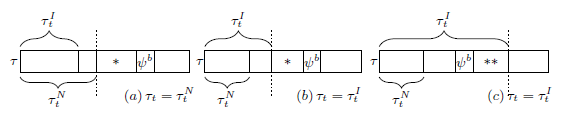
\includegraphics[width=\textwidth]{img/cases.png}
\caption{\label{fig:cases} Расположение $\tau^N_t, \tau^I_t, \psi^b$} 
\end{figure}
Докажем, что след $\tau_{\psi} \in \llbracket P \rrbracket (s)$. Начнём с анализа построения следа $\tau_t$ при $t \neq t_0$. Рассмотрим три возможных варианта расположения $\tau^N_t$, $\tau^I_t$, $\psi^b$ относительно друг друга, изображенные на рисунке \ref{fig:cases}. В соответствии с выбором следа $\tau^N_t$ в случаях $(a)$ и $(b)$ фрагмент следа $\tau$ между концом $\tau^N_t$ и действием $\psi^b$ может содержать только транзакционные действия потока $t$. В соответствии с выбором следа $\tau^I_t$ и $\psi^b$ в случае $(c)$ фрагмент следа $\tau$ между действием $\psi^b$ и концом $\tau^I_t$ не может содержать действие $txbegin$ потока t. Из-за выбора $\tau^N_t$ данный фрагмент содержит только транзакционные действия потока $t$. Более того эти действия принадлежат либо транзакции, запущенной действием $\psi^b$, либо транзакции, которая была запущена до действия $\psi^b$. В соответствии с выбором $\psi^b$ за $\psi^b$ следуют только транзакционные действия потока $t_0$, которые принадлежат либо транзакции, запущенной действием $\psi^b$, либо транзакции, которая была запущена до действия $\psi^b$. Из данного анализа следует, что преобразования следа $\tau$ в $\tau'$ состоит из двух действий:
\begin{enumerate}[label=(\roman*)]
\item Удаление действий, следующих за действием $\psi^b$, за исключением действий уже запущенных транзакций.
\item Удаление некоторых суффиксов потоков, содержащих только транзакционные действия. 
\end{enumerate}
Так как у транзакций нет доступа к глобальным переменным, то на них не влияют действия других потоков. Согласно определению множества $A'(P)$ (рисунок \ref{fig:actions}), множество $\llbracket P\rrbracket(s)$ содержит префиксы следа $\tau \in \llbracket P\rrbracket(s)$. Следовательно, $\tau' \in \llbracket P\rrbracket(s)$.

Покажем, что след $\tau''$ корректен, ссылаясь на случаи $(a-c)$. Пусть $T = txof(\psi^b, H_1\psi)$, тогда $T \in H'_1\psi$ из-за выбора действия $\psi^b$. По определению \ref{def1}(iii) % изменить ссылку
получаем \eqref{eq:transform4iii}. Следовательно, в случаях $(a)$ и $(b)$ $\tau'|_t$ не содержит прерванных транзакций, которые принадлежат $H'_1\psi$. В случае $(c)$ прерванная транзакция, принадлежащая $H'_1\psi$, может быть только последней транзакцией $\tau'|_t$. Как было доказано выше, $(H'_1\psi)|_{t_0}$ не содержит прерванных транзакций. Следовательно, за прерванными транзакциями следа $\tau'$, чей статус был изменён при построении $\tau''$, нет действий. Кроме того, $\llbracket P\rrbracket(s)$ допускает произвольное прерывание и фиксацию транзакций. Следовательно, $\tau'' \in \llbracket P\rrbracket(s)$. Так как след $\tau_{\psi}$ получен из следа $\tau''$ фиксацией транзакций, находящихся в ожидании фиксации, а $\llbracket P\rrbracket(s)$ допускает произвольную фиксацию транзакций, то  $\tau_{\psi} \in \llbracket P\rrbracket(s)$.

Наконец, покажем, что $history(\tau_{\psi})|_{\neg abortedtx} = H^c_{\psi}$. Так как $\tau_{\psi} = \tau''H^{cc}$, и $H^{cc}$ содержит только зафиксированные действия, тогда достаточно показать, что $history(\tau'')|_{\neg abortedtx} = H''_1\psi$. Получаем, что
\begin{align*}
history(\tau_{\psi})|_{\neg aborted} = &\quad history(\tau''H^{cc})|_{\neg aborted} = \\
                                 &\quad history(\tau'')|_{\neg abortedtx}H^{cc} = H''_1{\psi}H^{cc} =H^c_{\psi}.
\end{align*}
В соответствии с выбором $\tau^I_t$ для $t \neq t_0$ каждая транзакция в $(H'_1\psi)|_t$ также находится в $\tau^I_t$. Следовательно $H'_1\psi$ --- подпоследовательность истории $history(\tau')$. По определению $\tau''$ и $H''_1$, $H''_1\psi$ --- подпоследовательность $history(\tau'')$. Так как $H''_{\psi}$ не содержит прерванных транзакций, то $H''_1\psi$ --- подпоследовательность $history(\tau'')|_{\neg abortedtx}$.

Для того, чтобы доказать, что $history(\tau'')|_{\neg abortedtx} = H''_1\psi$, осталось показать, что каждая не прерванная транзакция в $history(\tau'')$ содержится в $H''_1\psi$. Так как след $\tau''$ получен из следа $\tau'$ изменением статуса транзакций, принадлежащих истории $H'_1\psi$, достаточно показать, что каждая не прерванная транзакция в $history(\tau')$ содержится в $H'_1\psi$. Рассмотрим все возможные случаи:
\begin{itemize}
\item[--] Рассмотрим поток $t \neq t_0$ и $\tau'|_t = \tau^N_t \neq \varepsilon$. Пусть $\chi^N_t$ --- последнее действие в $\tau^N_t$ и $T = txof(\psi^b, H_1\psi) \in H'_1\psi$. По определению \ref{def1}(iii) % изменить ссылку на определение
получаем \eqref{eq:transform4iii}. Так как $\chi^N_t$ предшествует действию $\psi^b$ в $H_1\psi$, то для любой транзакция $T'$, принадлежащей $\tau'|_t$, выполняется отношение $T' \prec_{H_1\psi} T$. Тогда согласно \eqref{eq:transform4iii}, если $T'$ --- зафиксированная транзакция, тогда она принадлежит $H'_1\psi$. Отсюда следует, что $history(\tau'')|_{\neg abortedtx} = H''_1\psi$.
\item[--] Рассмотрим поток $t \neq t_0$ и $\tau'|_t = \tau^I_t \neq \varepsilon$. Пусть $\psi^I_t$ --- последнее действие в $\tau^I_t$. Пусть $T = txof(\psi^I_t, H_1\psi)$. $T \in H'_1\psi$ в соответствии с выбором $\tau^I_t$. По определению \ref{def1} % изменить ссылку
получаем \eqref{eq:transform4iii}. Так как любая транзакция $T'$ из истории $history(\tau'|_t)$ является либо транзакцией $T$, либо $T' \prec_{(H_1\psi)|_t} T$, то из \eqref{eq:transform4iii} следует, что $history(\tau'')|_{\neg abortedtx} = H''_1\psi$.
\item[--] Рассмотрим поток $t = t_0$. Пусть $T = txof(\psi, H_1\psi) \in H'_1\psi$. Тогда по определению \ref{def1}(iii) % изменить ссылку на определение
получаем \eqref{eq:transform4iii}. Так как любая транзакция $T'$ из истории $history(\tau'|_{t_0})$ является либо транзакцией $T$, либо $T' \prec_{(H_1\psi)|_{t_0}} T$, то из \eqref{eq:transform4iii} следует, что $history(\tau'')|_{\neg abortedtx} = H''_1\psi$.
\end{itemize}
\end{myproof}
\begin{lemma}\label{sufficiency3}
Пусть H --- история, в которой все прерванные транзакции прерываются мгновенно, и S --- история такая, что $H|_{\neg abortedtx} \sqsubseteq_{op} S$. Тогда существует история $S' \in addab(S)$ такая, что $H \sqsubseteq_{op} S'$. 
\end{lemma}
\begin{myproof}
Пусть $n$ --- число прерванных транзакций истории $H$. Для построения истории $S'$ построим по индукции последовательность $S_i, i = 0 \ldots n$, для которой будут выполнятся следующие условия:
\begin{align}\label{eq:SiInduct}
\begin{split}
|aborted(S_i)| = i; \; S_i \in addab(S); \; \{\psi| \psi \in S_i\} \subseteq \{\psi | \psi \in H \}; \\ \forall \; \psi_1, \psi_2 \in S_i: \psi_1 \prec_H \psi_2 \implies \psi_1 \prec_{S_i} \psi_2.
\end{split}
\end{align}

Пусть для $i = 0$ $S_0 = S$ и все требования \eqref{eq:SiInduct} выполнены. Предположим, что $S_i$ удовлетворяет требованиям \eqref{eq:SiInduct}. Построим $S_{i+1}$ из $S_i$. Пусть $H = H_1\psi_{b}H_2\psi_{a}H_3$, где $\psi_b = (\_, t, txbegin)$, $\psi_a = (\_,t, aborted)$, $H_2|_t = \varepsilon$ и $$\neg \; \exists \; \psi' \; \psi' = (\_, \_, txbegin) \in H_1 \land txof(\psi', H) \in aborted(H) \land \psi' \notin S_i.$$

Транзакция $\psi_b\psi_a$ --- первая транзакция в истории H, которая не принадлежит $S_i$. Рассмотрим два случая:
\begin{itemize}
\item[--] $H_1$ не содержит $committed$ или $aborted$ действий. Пусть $S_{i+1} = \psi_b\psi_{a}S_i$. Нужно показать, что для любого $\psi' \in S_i$ выполняется $\psi' \prec_H \psi_b \implies \psi' \prec_{S_{i+1}} \psi_b$ или $\psi_a \prec_H \psi' \implies \psi_a \prec_{S_{i+1}} \psi'$. Согласно конструкции $S_{i+1}$ выполняется последнее условие. $H_1$ не может содержать $committed$ или $aborted$ действий, поэтому $H_1$ не содержит действий потока $t$. Следовательно, отношение $\psi' \prec_H \psi_b$ не выполняется для любого $\psi'$. 
\item[--] $H_1$ содержит $committed$ или $aborted$ действия. Пусть $\psi$ --- последнее $committed$ или $aborted$ действие в $S_i$, которое также принадлежит $H_1$. Пусть $S_{i} = S'\psi{S''}$, $S_{i+1} = S'\psi\psi_b\psi_a{S''}$. Покажем, что для любого $\psi' \in S_i$ выполняется $\psi' \prec_H \psi_b \implies \psi' \prec_{S_{i+1}} \psi_b$ или $\psi_a \prec_H \psi' \implies \psi_a \prec_{S_{i+1}} \psi'$.

Предположим, что $\psi' \prec_{H} \psi_b$ для $\psi' \in S_i$, тогда $\psi' \in H_1$. В соответствии с выбором $\psi_b$, $\psi_a$, $\psi$ все $committed$ и $aborted$ действия из $H_1$ принадлежат $S'\psi$. Если $\psi'$ --- $committed$ или $aborted$ действие, тогда $\psi' \in S'\psi$. Из построения $S_{i+1}$ следует, что $\psi' \prec_{S_{i+1}} \psi_b$. Если $\psi'$ --- действие потока $t$, тогда $\psi'$ либо $committed$ или $aborted$ действие, либо $\psi'$ предшествует такому действию $\psi'' \in S_i$ потока $t$ в $H_1$: $\psi' \prec_{H_1} \psi''$. Тогда $\psi' \prec_{S'\psi} \psi''$ и $\psi' \prec_{S_{i+1}} \psi''$. Следовательно, $\psi'' \prec_{S_{i+1}} \psi_b$ и $\psi' \prec_{S_{i+1}} \psi_b$. 

Предположим, что $\psi_a \prec_{H} \psi'$ для $\psi' \in S_i$, тогда $\psi' \in H_3$. Если $\psi' = (\_,\_, txbegin)$, тогда $\psi \prec_{H} \psi'$. Так как для $S_i$ выполняются условия \eqref{eq:SiInduct}, то $\psi \prec_{S_i} \psi'$ и $\psi' \in S''$. Тогда из построения $S_{i+1}$ следует, что $\psi_a \prec_{S_{i+1}} \psi'$. Если $\psi'$ --- действие потока $t$, тогда $\psi'$ либо $txbegin$ действие, либо $\psi'$ следует за $txbegin$ действием $\psi'' \in S_i$ потока $t$ в $H_3$: $\psi'' \prec_{H_3} \psi'$ и $\psi'' \prec_{S_i} \psi'$. Так как $\psi \in H_1$, то $\psi \prec_H \psi''$. Из этого следует, что $\psi \prec_{S_i} \psi''$, $\psi'', \psi' \in S''$ и $\psi'' \prec_{S_{i+1}} \psi'$. Из построения $S_{i+1}$ следует, что $\psi_a \prec_{S_{i+1}} \psi''$. Следовательно, $\psi_a \prec_{S_{i+1}} \psi'$. 
\end{itemize}

\end{myproof}
\begin{lemma}\label{sufficiency4}
Если $\mathcal{T}_C \sqsubseteq_{tms} \mathcal{T}_A$ и $\mathcal{T}_A$ удовлетворяет 1 и 2 свойствам замкнутости, тогда $\forall \; \tau \in \llbracket P, \mathcal{T}_C\rrbracket(s)$ $\exists \; \tau' \in \llbracket P, \mathcal{T}_A \rrbracket(s)$ такие, что $(\tau'|_{\neg trans} = \tau|_{\neg trans}) \land (\forall \; t \; (\tau'|_t)|_{obs} = (\tau|_t)|_{obs})$.\end{lemma}
\begin{myproof}
Пусть $H = history(\tau)$. По предположению леммы $\mathcal{T}_C \sqsubseteq_{tms} \mathcal{T}_A$. Следовательно $\exists \; H^c \in comp(H)|_{\neg live}$ и $\exists \; S \in \mathcal{T}_A$ такие, что $H^c|_{com} \sqsubseteq_{op} S$. Тогда $H^c = (H|_{\neg live})H'$, для некоторой последовательности действий $H'$, состоящей из $committed$ и $aborted$ действий.  Пусть $\tau^c = \tau_0H'$, где след $\tau_0$ получен из следа $\tau$ удалением всех действий действующих транзакций. Следовательно, $history(\tau^c) = H^c$.

Покажем, что $\tau^c \in \llbracket P \rrbracket(s)$. Согласно определению множества $A'(P)$ (рисунок \ref{fig:actions}), множество $\llbracket P\rrbracket(s)$ содержит префиксы следа $\tau \in \llbracket P\rrbracket(s)$. Кроме того, $\llbracket P\rrbracket(s)$ допускает произвольное прерывание и фиксацию транзакций. Так как след $\tau^c$ получен из $\tau$ удалением только некоторых последних транзакций потоков и завершением транзакций, ожидающих фиксацию, то $\tau^c \in \llbracket P\rrbracket(s)$. Кроме того, $\tau^c|_{\neg trans} = \tau|_{\neg trans}$ и $(\tau|_t)|_{obs}$ --- префикс $(\tau^c|_t)|_{obs}$. Пусть $\tau^{na} = \tau^c|_{\neg abortact}$. Согласно утверждению 1 % добавить утверждение и ссылку
$\tau^{na} \in \llbracket P \rrbracket(s)$. Так как $(H^c|_{\neg abortact})|_{\neg abortedtx} = H^c|_{com} \sqsubseteq_{op} S$, то по лемме \ref{sufficiency3} % добавить лемму 3 и ссылку
существует история $S' \in addab(S)$ такая, что $history(\tau^{na}) = H^c|_{\neg abortact} \sqsubseteq_{op} S'$. Так как $S \in \mathcal{T}_A$ и $\mathcal{T}_A$ замкнута относительно мгновенного прерывания транзакций, то $S' \in \mathcal{T}_A$. Так как $\tau^{na} \in \llbracket P \rrbracket(s)$, тогда по лемме 2 % добавить лемму 2 и ссылку
существует след $\tau'' \in \llbracket P \rrbracket(s)$ такой, что $history(\tau'') = S',$ $$\tau''|_{\neg trans} = \tau^{na}|_{\neg trans} = \tau^c|_{\neg trans} = \tau|_{\neg trans},$$
и $\tau''|_t = \tau^{na}|_t$. Пусть $\tau'$ --- след, полученный из $\tau''$ удалением последних ответов на запросы каждого потока в $H'$. Тогда $$\tau'|_{\neg trans} = \tau''|_{\neg trans} = \tau|_{\neg trans},$$ $\tau' \in \llbracket P\rrbracket(s)$. Так как $\mathcal{T}_A$ замкнута относительно удаления ответов на запросы, то $history(\tau') \in \mathcal{T}_A$.

Покажем, что $(\tau'|_t)|_{obs} = (\tau|_t)|_{obs}$. Так как $\tau''|_t = \tau^{na}|_t$, то $$(\tau''|_t)|_{obs} = (\tau^{na}|_t)|_{obs} = ((\tau^c|_{\neg abortact})|_t)|_{obs} = (\tau^c|_t)|_{obs}.$$ Следовательно, $(\tau|_t)|_{obs}$ --- префикс $(\tau''|_t)|_{obs}$. След $\tau'$ получен из следа $\tau''$ удалением действий $H'$. Из этого следует, что $(\tau|_t)|_{obs} = (\tau'|_t)|_{obs}$.
\end{myproof}
  
\section{Доказательство теоремы 1 (ii) (Необходимость)}
\begin{lemma}\label{necessity1}
Пусть $\mathcal{T}_C$ и $\mathcal{T}_A$ --- конкретная и абстрактная транзакционная память такие, что $\mathcal{T}_C \preceq \mathcal{T}_A$ и $\mathcal{T}_A$ удовлетворяет 3 и 4 свойствам замкнутости. Тогда $\forall H \in \mathcal{T}_C$ $\exists H^c \in comp(H |_{\neg live})$, $S \in \mathcal{T}_A$: $H^c|_{com} \, \sqsubseteq_{op} S$.
\end{lemma}
\begin{myproof} Выберем целое значение $u \neq 1$, которого нет в $H$. Введем следующие обозначения:
\begin{itemize}
\item[--] $m$ --- наибольший идентификатор потока, встречающийся в $H$. 
\item[--] $k^t$ --- число транзакций потока $t$ в $H$, то есть число $(\_,t,txbegin)$ действий в $H$. 
\item[--] Разделим $H|_t$ на $k^t$ подпоследовательностей: $H|_t$ = $H^t_{1} \ldots H^t_{k^t}$, где $H^t_i$ состоит из действий $i$ транзакции потока $t$, $H^t_i(1)$ = $(\_,t, txbegin)$.
\item[--] $c^t_i$ --- результат $i$ транзакции потока $t$, то есть $c^t_i = committed$ или $c^t_i = aborted$. Если транзакция не завершена, то значение $c^t_i$ не определено.
\item[--] $q^t_i$ --- число $call$ действий в $H^t_i$.
\item[--] $(\_,t, call \, o^t_{i,j}.f^t_{i,j}(n^t_{i,j}))$ --- $j$ $call$ действие в $H^t_i$. 
\item[--] $(\_,t, ret(r^t_{i,j}) \, o^t_{i,j}.f^t_{i,j})$ --- $j$ $ret$ действие в $H^t_i$. Если запрос $(\_,t, call \, o^t_{i,j}.f^t_{i,j}(n^t_{i,j}))$ завершается прерыванием транзакции, тогда $r^t_{i,j}$ = $aborted$. Если нет ответа на запрос, то есть транзакция действующая и $(\_,t, call \, o^t_{i,j}.f^t_{i,j}(n^t_{i,j}))$ --- последнее действие, тогда $r^t_{i,j}$ = $u$.
\item[--] $lasttx(t, i, t')$ --- число завершенных транзакций потока $t'$ в $H$ до начала $i$ транзакции потока $t$, то есть число $(\_,t', committed)$ и $(\_,t', aborted)$ действий предшествующих $H^t_{i}(1)$ = $(\_,t,txbegin)$ действию.
\end{itemize}
\begin{figure}
\begin{flalign*}
 GP^t_i  &= z^t_{i,1} := g^1_{lasttx(t,i,1)}; if \left(z^t_{i,1} \neq 1 \right) then \, fault; \\
 &\mathrel{\phantom{=}} \ldots \\ 
 &\mathrel{\phantom{=}} z^t_{i,m} := g^m_{lasttx(t,i,m)}; if \left(z^t_{i,m} \neq 1 \right) then \, fault
\end{flalign*}
\begin{itemize}
\item[--] Если $H^t_{i}$ --- зафиксированная транзакция или прерванная и видимая транзакция, тогда
\begin{alignat}{2}
     CP^t_i =&\quad \omega^t_{i} := &\; atomic\{&y^t_{i,1} := o^t_{i,1}.f^t_{i,1}(n^t_{i,1}); \; if \left (y^t_{i,1} \neq r^t_{i,1}\right) then \; fault; \nonumber \\
         &           &&\ldots \nonumber \\
         &           &&y^t_{i,q^t_i} := o^t_{i,q^t_i}.f^t_{i,q^t_i}(n^t_{i,q^t_i}); \; if \left (y^t_{i,q^t_i} \neq r^t_{i,q^t_i}\right) then \; fault\} \nonumber \\
         &\quad \mathrlap{if \left(\omega^t_{i} \neq c^t_{i} \right) then \; fault \; else \; g^t_{i} := 1} \nonumber
\end{alignat}
\item[--] Если $H^t_{i}$ --- действующая транзакция или прерванная и не видимая транзакция, тогда
\begin{alignat}{2}
     CP^t_i =&\quad \omega^t_{i} := &\; atomic\{&y^t_{i,1} := o^t_{i,1}.f^t_{i,1}(n^t_{i,1}); \nonumber \\
         &           &&\ldots \nonumber \\
         &           &&y^t_{i,q^t_i} := o^t_{i,q^t_i}.f^t_{i,q^t_i}(n^t_{i,q^t_i}); \nonumber \\
         &           &&fault \} \nonumber
\end{alignat}
\item[--] Если $H^t_{i}$ --- ожидающая фиксации транзакция, тогда 
\begin{alignat}{2}
     CP^t_i =&\quad \omega^t_{i} := &\; atomic\{&y^t_{i,1} := o^t_{i,1}.f^t_{i,1}(n^t_{i,1}); \; if \left (y^t_{i,1} \neq r^t_{i,1}\right) then \; fault; \nonumber \\
         &           &&\ldots \nonumber \\
         &           &&y^t_{i,q^t_i} := o^t_{i,q^t_i}.f^t_{i,q^t_i}(n^t_{i,q^t_i}); \; if \left (y^t_{i,q^t_i} \neq r^t_{i,q^t_i}\right) then \; fault\} \nonumber
\end{alignat}
\end{itemize}
\caption{Построение $GP^t_i$ и $CP^t_i$ команд}
\label{fig:commands}
\end{figure}
Для каждого потока $t$ = $1..m$ построим последовательность команд $$C^t_H = GP^t_1;CP^t_1;GP^t_2;CP^t_2;\ldots;GP^t_{k^t};CP^t_{k^t},$$ где $GP^t_i$ и $CP^t_i$ определены на рисунке ~\ref{fig:commands}.
Переменные $g^t_i$ --- глобальные, все остальные переменные --- локальные. Переменная $g^t_i$ используется для мониторинга порядка выполнения транзакций. Значение $g^t_i$ изменяется только потоком $t$ и используется для оповещения о завершении $i$ транзакции потока $t$. Переменная $z^t_{i,t'}$ используется для записи завершения $lasttx(t, i, t')$ транзакции потока $t'$, предшествующей запуск $i$ транзакции потока $t$. Так как значение $lasttx(t, i, t')$ может быть равно нулю, введём фиктивную переменную $g^t_0$ для каждого потока $t$. Переменная $\omega^t_i$ хранит информацию о статусе завершения $i$ транзакции потока $t$ (committed или aborted). Переменная $y^t_{i,j}$ записывает результат $j$ вызова метода объекта в $i$ транзакции потока $t$. 

Команда $GP^t_i;CP^t_i$ начинается с чтения сигналов ($g^t_{lasttx(t,i,t')}$) последней транзакции каждого потока $t'$, завершённой до начала $i$ транзакции потока $t$. Далее выполняется атомарный блок, в котором вызывается последовательность методов объектов транзакцией $H^t_i$. После завершения атомарного блока команда объявляет завершение транзакции. Определим программу $P_H$ следующим образом: $$P_H = C^1_H \; \parallel \ldots \parallel C^m_H.$$

Далее построим след $\tau$ программы $P_H$. Для начала построим $\tau^t$ для каждой последовательной команды $C^t_H$. Рассмотрим множество следов $A(C^t_H)t$ команды $C^t_H$, и пусть $\tau^t \in A(C^t_H)t$ --- максимальный след без $fault$ команды такой, что $H|_t$ = $history(\tau^t)$. След $\tau^t$ существует в связи с конструкцией $C^t_H$ и определением множества следов последовательной команды (рисунок \ref{fig:actions}). Во множестве $A(C^t_H)t$ существует след для каждого возможного параметра, результата вызова метода объекта и атомарного блока в $C^t_H$. В частности, $A(C^t)$ содержит след, в котором параметры, результат вызова методов объектов и атомарного блока такие же, как и в $H|_t$. Далее разделим каждый след $\tau^t$ на $|H|_t|$ подпоследовательностей: 
\begin{equation}\label{eq:tau_t}
\tau^t = \tau^t_1\ldots\tau^t_{|H|_t|}.
\end{equation}
Для каждого потока $i$ = $1..|H|_t|$ существует одно действие интерфейса $\psi^t_i$ в $\tau^t_i$, и выполняются условия, изображенные на рисунке \ref{fig:subtraces}. Это определяет след $\tau^t_i$ единственным образом и гарантирует, что, если след $\tau^t_i$ заканчивается $\psi^t_i = (\_,t,txbegin)$, то он содержит все действия, которые используются для чтения сигнализирующих глобальных переменных, предшествующих действию $\psi^t_i$ в $\tau^t$. Желаемый след строится с помощью чередования подпоследовательностей следов $\tau^1,\ldots,\tau^m$ согласно порядку, обусловленному историей $H$. Формально 
\begin{equation}\label{eq:tau}
\tau = \tau^{t_1}_{j_1} \ldots \tau^{t_{|H|}}_{j_{|H|}},
\end{equation}
где $H(i)$ = $(\_, t_i, \_)$ и $j_i$ = $|(H \downharpoonleft_i)|_{t_i}|.$ По построения $history(\tau)$ = $H$.
\begin{figure}
\begin{align*}
  \tau^t_i=\begin{cases}
    \_\psi^t_i, & \psi^t_i \in \{(\_,t,txbegin), (\_,t,call \; o.f(n)), (\_,t, txcommit)\};\\
    \psi^t_i, & \psi^t_i = (\_,t, OK); \\
    \psi^t_i(\_,t,y^t_{i,\_} := n), & \psi^t_i = (\_,t, ret(n) \; o.f) \land txof(\psi^t_i, \tau^t) \in live(\tau^t); \\
    \mathrlap{\psi^t_i(\_,t,y^t_{i,\_} := n)(\_,t,assume(y^t_{i,\_} = r^t_{i,\_})),}\\
                                    & \psi^t_i = (\_,t, ret(n) \; o.f) \land txof(\psi^t_i, \tau^t) \notin live(\tau^t); \\
    \mathrlap{\psi^t_i(\_,t,\omega_i := c^t_i)(\_,t,assume(\omega_i = c^t_i))(\_,t,g^t_i := 1),}\\
                                    & \psi^t_i \in \{(\_,t,committed), (\_,t,aborted))\}.       
  \end{cases}
\end{align*}
\caption{Построение $\tau^t_i$}
\label{fig:subtraces}
\end{figure}
Так как $\tau^t \in A(C^t_H)t$, то $\tau \in A(P_H)t$. Пусть $s$ --- состояние программы, в которой все локальные переменные инициализированы целым числом $u$, а глобальные переменные $g^t_i = 0$ при $i \neq 0$ и $g^t_0 = 1$. $eval(s,\tau) \neq \emptyset$ по построению $\tau$. Так как $history(\tau) = H \in \mathcal{T}_C$, то $\tau \in \llbracket P_H \rrbracket(s,\mathcal{T}_C)$. Так как $\tau \in \llbracket P_H \rrbracket(s,\mathcal{T}_C)$ и $\mathcal{T}_C \preceq \mathcal{T}_A$, то по определению \ref{def1} % изменить ссылку на опр 
существует след $\tau' \in \llbracket P_H \rrbracket(s,\mathcal{T}_A)$ такой, что $\tau'|_{\neg trans}$ = $\tau|_{\neg trans}$ и $S_1 = history(\tau') \in \mathcal{T}_A$.

Пусть $T$ и $T'$ --- $i$ транзакции потока $t$ в $\tau|_t$ и $\tau'|_t$ соответственно. Так как $\tau'|_{\neg trans}$ = $\tau|_{\neg trans}$, то либо транзакции $T$ и $T'$ запускается одинаковыми командами, либо $T'$ не существует. Проанализируем зависимость между этими транзакциями, основываясь на конструкции команды $C^t_H$ (рисунок \ref{fig:commands}):
\begin{itemize}
\item[--] Если транзакция $T$ завершена, тогда транзакция $T'$ тоже завершена, так как после завершения транзакции переменной $g^t_i$ присваивается новое значение и $\tau'|_{\neg trans}$ = $\tau|_{\neg trans}$. Завершённая транзакция $T$ --- зафиксированная тогда и только тогда, когда $T'$ --- зафиксированная. В данном случае проверки, выполненные внутри соответствующих атомарных блоков, доказывают, что возвращаемые результаты транзакционных действий внутри $T$ и $T'$ совпадают.
% может заменить слово доказывает на утверждает ?
\item[--] Если транзакция $T$ --- действующая, тогда присутствие команды $fault$ до завершения атомарного блока доказывает, что транзакция $T'$ может быть действующей, прерванной или не существовать. 
\item[--] Если транзакция $T$ ожидает фиксацию, тогда у транзакции $T'$ может быть любой статус, или она может не существовать. Однако, если $T$  --- видимая, тогда проверки внутри атомарного блока доказывают, что результаты транзакционных действий внутри $T$ и $T'$ совпадают.
\end{itemize}

Пусть $H_1 = (H|_{\neg live})|_{\neg abortedtx}$ и $S_2 = (S_1|_{\neg live})|_{\neg abortedtx}$. Так как $S_1 \in \mathcal{T}_A$ и $\mathcal{T}_A$ замкнута относительно операции удаления действующих и прерванных транзакций, то $S_2 \in \mathcal{T}_A$. Пусть $p'_t$ и $p''_t$ --- индексы последних $txcommit$ или $committed$ действий в $H_1|_t$ и $S_2|_t$ соответственно. В случае отсутствия этих действий, индексы равны 0. Пусть $p_t=min(p'_t,p''_t)$. Из приведенного анализа следует, что $\forall \; t \; (H_1|_t)\downharpoonleft_{p_t} \equiv (S_2|_t)\downharpoonleft_{p_t}$. Пусть $S_3$ --- история, полученная из $S_2$ переименованием идентификаторов действий таким образом, что $S_3 \equiv S_2$, $\forall \; t \; (H_1|_t)\downharpoonleft_{p_t} = (S_3|_t)\downharpoonleft_{p_t}$, и все действия в $S_3$, которые не принадлежат $(S_2|_t)\downharpoonleft_{p_t} \; \forall \; t$, имеют идентификаторы, которые не встречаются в $H$. Так как $S_2 \in \mathcal{T}_A$ и $\mathcal{T}_A$ замкнута относительно операции переименования идентификаторов, то $S_3 \in \mathcal{T}_A$.

Так как $S_3 \in \mathcal{T}_A$ и $\mathcal{T}_A$ --- замкнута относительно операции завершения транзакций, ожидающих фиксации, получаем, что существует история $S_4 \in nicomp(S_3) \cap \mathcal{T}_A$. Пусть $S'_3$ --- подпоследовательность $S_4$, которая содержит только $committed$ или $aborted$ действия, которых нет в $S_3$. % т.е. эти действия - завершение транз
Идентификаторы действий в $S'_3$ не встречаются в $H$. Пусть $S''_3$ --- подпоследовательность $committed$ действий в $S_3$, которых нет в $H_1$. Построим требуемую историю $H^c$ с помощью прерывания всех ожидающих фиксацию транзакций истории $(H|_{\neg live})S''_3S'_3$. Пусть $H^c = (H|_{\neg live})S''_3S'_3H_a$, где $H_a$ состоит из действий $(\_, t, aborted)$ для каждого потока $t$, который завершается транзакцией, ожидающей фиксации, в $(H|_{\neg live})S''_3S'_3$. У этих действий есть уникальные идентификаторы, которые не появляются в $H$. $H^c \in comp(H|_{\neg live})$ по следующим причинам: 
\begin{enumerate}[label=(\roman*)]
\item $S''_3$ завершает транзакции, зафиксированные в $S_1$, но ожидающие фиксацию в $H$.  
\item $S'_3$ завершает транзакции, ожидающие фиксацию в $H$ и $S_1$.
\item $H_a$ прерывает транзакции, ожидающие фиксацию в $H$, которые могут быть действующими, прерванными или не существовать в $S_1$.
\end{enumerate}

Пусть $S = S_4|_{com}$. $S \in \mathcal{T}_A$, так как $S_4 \in \mathcal{T}_A$ содержит только завершенные транзакции, и транзакционная память $\mathcal{T}_A$ замкнута относительно удаления действующих и прерванных транзакций. Докажем, что $H^c|_{com} \sqsubseteq_{op} S$. Для начала покажем, что $\forall \; t \; (H^c|_t)|_{com} = S|_t$, рассмотрев следующие случаи:
\begin{itemize}
\item[--] $H|_t$ не содержит транзакций, ожидающих фиксацию. Тогда $p'_t = p''_t$, $H_1|_t = S_3|_t$ и $S'_3 = S''_3 = H_a = \varepsilon$. Следовательно, $$(H^c|_t)|_{com} = (H_1|_t)|_{com} = (S_3|_t)|_{com} = (S_4|_t)|_{com} = S|_t.$$
\item[--] $H|_t$ завершается транзакцией, ожидающей фиксацию, и $(S''_3S'_3H_a)|_t = S''_3|_t = (\_,t,committed)$. Тогда $H_1|_t = (H_1|_t)\downharpoonleft_{p_t}$ и $S_3|_t = ((S_3|_t)\downharpoonleft_{p_t})(S''_3|_t)$. Следовательно, 
\begin{align*}
(H^c|_t)|_{com} = ((H_1|_t)(S''_3|_t))|_{com} = (((H_1|_t)\downharpoonleft_{p_t})(S''_3|_t))|_{com} = \\
(((S_3|_t)\downharpoonleft_{p_t})(S''_3|_t))|_{com} = (S_3|_t)|_{com} = (S_4|_t)|_{com} = S|_t.
\end{align*}
\item[--] $H|_t$ завершается транзакцией, ожидающей фиксацию, и $(S''_3S'_3H_a)|_t = S'_3|_t$. Тогда $H_1|_t = S_3|_t$, так как $p'_t = p''_t$. Следовательно, 
\begin{align*}
(H^c|_t)|_{com} = ((H_1|_t)(S'_3|_t))|_{com} = ((S_3|_t)(S'_3|_t))|_{com} = (S_4|_t)|_{com} = S|_t.
\end{align*}
\item[--] $H|_t$ завершается транзакцией, ожидающей фиксацию, и $(S''_3S'_3H_a)|_t$ = $H_a|_t$ = $(\_, t, aborted)$. Тогда $((H_1|_t)(H_a|_t))|_{com} = ((H_1|_t)\downharpoonleft_{p_t})|_{com}$ и $S_3|_t = (S_3|_t)\downharpoonleft_{p_t}$. Следовательно,
\begin{align*}
(H^c|_t)|_{com} = ((H_1|_t)(H_a|_t))|_{com} = ((H_1|_t)\downharpoonleft_{p_t})|_{com} =\\
((S_3|_t)\downharpoonleft_{p_t})|_{com} = (S_3|_t)|_{com} = (S_4|_t)|_{com} = S|_t. 
\end{align*}
\end{itemize}

Эти рассуждения доказывают, что $\forall \; t \; (H^c|_t)|_{com} = S|_t$. Для каждой завершённой транзакции $T$ в $\tau$ значение $g^t_i = 1$, и значение этой переменной читается до начала транзакции $T'$, которая запускается после завершения $T$. Следовательно транзакция в $\tau'$, соответствующая $T$, завершается до начала транзакции в $\tau'$, соответствующей $T'$. Следовательно порядок выполнения транзакций в $H^c$ сохраняется в $S$, откуда следует, что $H^c|_{com} \sqsubseteq_{op} S$. 
\end{myproof}
\begin{lemma}\label{necessity2}
Пусть $\mathcal{T}_C$ и $\mathcal{T}_A$ --- конкретная и абстрактная транзакционная память такие, что $\mathcal{T}_C \preceq \mathcal{T}_A$ и $\mathcal{T}_A$ удовлетворяет 3 и 4 свойствам замкнутости. Пусть $H = H'\psi$, где $\psi$ --- ответ на запрос, при этом $\psi \notin \{(\_,\_,committed),(\_,\_,aborted)\}$. Тогда $\exists H^c \in cTMSpast(H)$ и $\exists S \in \mathcal{T}_A$ такие, что $H^c \sqsubseteq_{op} S$.
\end{lemma}
\begin{myproof}
Для доказательства данной леммы будут использованы ранее введенные обозначения. Для каждого потока $t$ = $1..m$ построим последовательность команд $$C^t_H = GP^t_1;CP^t_1;GP^t_2;CP^t_2;\ldots;GP^t_{k^t};CP^t_{k^t}.$$

\begin{figure}
\begin{flalign*}
 GP^t_i  &= z^{t_0}_{i,1} := g^1_{lasttx(t_0,i,1)}; if \left(z^{t_0}_{i,1} \neq 1 \right) then \, mismatch := 1; \\
 &\mathrel{\phantom{=}} \ldots \\ 
 &\mathrel{\phantom{=}} z^{t_0}_{i,m} := g^m_{lasttx(t_0,i,m)}; if \left(z^{t_0}_{i,m} \neq 1 \right) then \, mismatch := 1
\end{flalign*}
\begin{itemize}
\item[--] Для $i \neq k^{t_0}$ команда $CP^{t_0}_i$ построена следующим образом:
\begin{alignat}{2}
     CP^{t_0}_i =&\quad \omega^{t_0}_{i} := &\; atomic\{&y^{t_0}_{i,1} := o^{t_0}_{i,1}.f^{t_0}_{i,1}(n^{t_0}_{i,1}); \nonumber \\ 
     &&& if \left (y^{t_0}_{i,1} \neq r^{t_0}_{i,1}\right) then \; mismatch := 1; \nonumber \\
         &           &&\ldots \nonumber \\
         & && y^{t_0}_{i,q^{t_0}_i} := o^{t_0}_{i,q^{t_0}_i}.f^{t_0}_{i,q^{t_0}_i}(n^{t_0}_{i,q^{t_0}_i}); 
         \nonumber \\ 
         &&& if \left (y^{t_0}_{i,q^{t_0}_i} \neq r^{t_0}_{i,q^{t_0}_i}\right) then \; mismatch := 1\} \nonumber \\
         &\quad \mathrlap{if \left(\omega^{t_0}_{i} \neq c^{t_0}_{i} \right) then \; mismatch := 1 \; else \; g^{t_0}_{i} := 1} \nonumber
\end{alignat}
\item[--] Команда $CP^{t_0}_{k^{t_0}}$ построена следующим образом:
\begin{alignat}{2}
     CP^{t_0}_{k^{t_0}} =&\quad \omega^{t_0}_{k^{t_0}} := &\; atomic\{&y^{t_0}_{k^{t_0},1} := o^{t_0}_{k^{t_0},1}.f^{t_0}_{k^{t_0},1}(n^{t_0}_{k^{t_0},1}); \nonumber \\ 
     &&& if \left (y^{t_0}_{k^{t_0},1} \neq r^{t_0}_{k^{t_0},1}\right) then \; mismatch := 1; \nonumber \\
         &           &&\ldots \nonumber \\
         & && y^{t_0}_{k^{t_0},q^{t_0}_{k^{t_0}}} := o^{t_0}_{k^{t_0},q^{t_0}_{k^{t_0}}}.f^{t_0}_{k^{t_0},q^{t_0}_{k^{t_0}}}(n^{t_0}_{k^{t_0},q^{t_0}_{k^{t_0}}}); 
         \nonumber \\ 
         &&& if \left (y^{t_0}_{k^{t_0},q^{t_0}_{k^{t_0}}} \neq r^{t_0}_{k^{t_0},q^{t_0}_{k^{t_0}}}\right) then \; mismatch := 1 \nonumber \\
         &&& if \left(mismatch \neq 1 \right) then \; fault \} \nonumber
\end{alignat}
\end{itemize}
\caption{Построение $GP^{t_0}_i$ и $CP^{t_0}_i$ команд}
\label{fig:commands_t0}
\end{figure}

Пусть $\psi = (\_,t_0,\_)$. Для $t \neq t_0$ $GP^t_i$ и $CP^t_i$ определены на рисунке ~\ref{fig:commands}, а для $t = t_0$ $GP^t_i$ и $CP^t_i$ определены на рисунке ~\ref{fig:commands_t0}. Для проверки результатов вызовов методов объектов транзакционной памяти в потоке $t_0$ используется локальная переменная $mismatch$. Если результат не соответствует $H|_{t_0}$, тогда поток $t_0$ в программе $P_H$ устанавливает значение переменной $mismatch$ равным единице, $mismatch = 1$. В конце выполнения программы поток проверяет значение этой переменной и прерывает выполнение, если локальные наблюдения потока $t_0$ совпадают с историей $H|_{t_0}$, то есть $mismatch \neq 1$.

Для того чтобы построить след $\tau$ программы $P_H$, построим след $\tau^t$ для каждой команды $C^t_H$, $t = 1..m$. Рассмотрим множество следов $A(C^t_H)$. Пусть $\tau^t \in A(C^t_H)$ --- максимальный след в $A(C^t_H)$ такой, что $H|_t = history(\tau^t)$. След $\tau^{t_0}$ завершается командой $fault$. Далее разделим каждый след $\tau^t$ на $|H|_t|$ подпоследовательностей, как было определено в формуле \eqref{eq:tau_t}. Условия, изображенные на рисунке \ref{fig:subtraces}, изменяются для случая $t=t_0$ и $\psi^{t_0}_i = \psi$:
\begin{align}
\tau^t_i = &\quad \psi(\_, t, y^t_{i,\_} := n)(\_, t, assume(y^t_{i,\_} = \nonumber \\
&\qquad \qquad r^t_{i,\_}))(\_, t, assume(mismatch \neq 1))(\_, t, fault). \nonumber
\end{align}
Желаемый след $\tau$ строится с помощью чередования подпоследовательностей следов $\tau^1,\ldots,\tau^m$ согласно порядку, обусловленному историей $H$, как было определено в формуле \eqref{eq:tau}. По построения $history(\tau)$ = $H$.

Так как $\tau^t \in A(C^t_H)t$, то $\tau \in A(P_H)t$. Пусть $s$ --- состояние программы, в которой все локальные переменные инициализированы целым числом $u$, а глобальные переменные $g^t_i = 0$ при $i \neq 0$ и $g^t_0 = 1$. $eval(s,\tau) \neq \emptyset$ по построению $\tau$. Так как $history(\tau) = H \in \mathcal{T}_C$, то $\tau \in \llbracket P_H \rrbracket(s,\mathcal{T}_C)$. Так как $\tau$ завершается $fault$ действием и $\mathcal{T}_C \preceq \mathcal{T}_A$, то по определению \ref{def1} % изменить ссылку на опр
существует след $\tau' \in \llbracket P_H \rrbracket(s,\mathcal{T}_A)$, который тоже завершается действием $fault$ потока $t_0$. $S_1 = history(\tau') \in \mathcal{T}_A$.

Так как оба следа $\tau$ и $\tau'$ завершаются командой $fault$ потока $t_0$, то проверки внутри потоков указывают на то, что \begin{equation} \label{eq:hist_fault}
(H|_{\neg abortedtx})|_{t_0} \equiv ({S_1}|_{\neg abortedtx})|_{t_0}. 
\end{equation}
Рассмотрим потоки $t \neq t_0$ и $t'$. Пусть $T$ и $T_1$ --- i транзакции в историях $H|_t$ и ${S_1}|_t$ соответственно. Пусть $T'$ и $T'_1$ --- j транзакции в историях $H|_{t'}$ и ${S_1}|_{t'}$ соответственно ($T_1$ и $T'_1$ могут не существовать). Из построения $P_H$ следует:
\begin{enumerate}
\item Так как $\tau$, $\tau'$ содержат только одну команду $fault$, то транзакция T не может быть действующей или прерванной, но не видимой (рисунок \ref{fig:commands}). Следовательно, если $T_1$ видимая транзакция, то транзакция $T$ тоже видимая. Кроме того, проверки внутри атомарных блоков доказывают, что результаты вызовов методов объектов в транзакциях $T$ и $T'$ совпадают.  
\item Если $T' \prec_H T$ и транзакция $T_1$ существует, тогда существует транзакция $T'_1$, и $T'_1 \prec_{S_1} T_1$, при этом $T'$ --- зафиксированная транзакция тогда и только тогда, когда $T'_1$ --- зафиксированная транзакция. Это обусловлено тем, что перед запуском транзакции $T_1$ в $\tau'$ осуществляется проверка равенства значения переменной $g^{t'}_j$ единице. $g^{t'}_j = 1$, если пройдены проверки внутри транзакции $T'_1$ и проверка статуса транзакции $T'_1$.   
\end{enumerate}

Пусть $S_2 = (S_1|_{\psi\cup{\neg live}})|_{\neg abortedtx}$, где $\cdot|_{\psi \cup {\neg live}}$ --- проекция на действия не действующих транзакций, за исключением транзакции действия $\psi$. Так как $S_1 \in \mathcal{T}_A$ и транзакционная память $\mathcal{T}_A$ замкнута относительно удаления действующих и прерванных транзакций, то $S_2 \in \mathcal{T}_A$. Так как $S_2 \in \mathcal{T}_A$ и $\mathcal{T}_A$ замкнута относительно завершения транзакций, ожидающих фиксацию, то существует история $S_3 \in nicomp(S_2) \cap \mathcal{T}_A$. Пусть $S_4 = S_3|_{\psi \cup com}$, где $\cdot|_{\psi \cup com}$ --- проекция на зафиксированные транзакции и транзакции действия $\psi$. Так как $S_3 \in \mathcal{T}_A$ не содержит транзакций, ожидающих фиксацию, и $\mathcal{T}_A$ замкнута относительно удаления действующих и прерванных транзакций, то $S_4 \in \mathcal{T}_A$.

Пусть $H_1$ --- подпоследовательность истории $H$, состоящая из транзакций, для которых соответствующие транзакции в $S_1$ включены в $S_4$. Следовательно, исходя из первого пункта приведённого выше анализа и формулы \eqref{eq:hist_fault} получаем: $$ tx(H_1) \subseteq \{txof(\psi,H) \} \cup visible(H).$$
Рассмотрим $T, T' \in tx(H_1)$ такие, что $T' \prec_{H_1} T$. Тогда существуют соответствующие им транзакции $T_1,T'_1 \in tx(S_1)$, из пункта 2 следует, что $T'_1 \prec_{S_1} T_1$. Из отношения $T'_1 \prec_{S_1} T_1$ следует, что $T'_1$ --- завершённая транзакция. В то же время транзакция $T'_1$ включена в историю $S_4$, которая содержит только зафиксированные транзакции и транзакцию $txof(\psi, S1)$. Отсюда следует, что $T'_1$ --- зафиксированная транзакция. Как было отмечено выше, $T'_1$ --- зафиксированная транзакция тогда и только тогда, когда $T'$ --- зафиксированная транзакция. Следовательно $T' \in committed(H)$. Докажем в обратную сторону. Рассмотрим $T \in tx(H_1)$, $T' \in committed(H)$ такие, что $T' \prec_H T$. Докажем, что $T' \in tx(H_1)$. Так как $T \in tx(H_1)$, то существует cоответствующая ей транзакция $T_1 \in tx(S_1)$. Тогда, как было отмечено выше, существует соответствующая $T'$ зафиксированная транзакция $T'_1 \in tx(S_1)$. Следовательно $T'_1 \in tx(S_4)$, и $T' \in tx(H_1)$. По определению допустимой истории $H_1 \in TMSpast(H)$. % сделать ссылку на определение 

Пусть $H_1 = H'_1\psi$, $H^c \in ccomp(com(H'_1)\psi)$. Тогда $H^c \in cTMSpast(H)$. Из равенства \ref{eq:hist_fault} следует, что $(H_1|_{t_0}) \equiv (S_4|_{t_0})$. Пусть $p_t$ --- индекс последнего $txcommit$ действия в $S_4|_t$ при $t \neq t_0$. Из пунктов 1 и 2 следует, что $(H_1|_{t})\downharpoonleft {p_t} \equiv (S_4|_{t})\downharpoonleft {p_t}$ для $t \neq t_0$. Так как история $H_1$ может содержать транзакцию, ожидающую фиксацию, которой будет соответствовать зафиксированная транзакция в $S_4$, то $H^c|_{t} \equiv S_4|_{t} \forall t$. Пусть $S$ --- история, полученная из $S_4$ переименованием идентификаторов действий таким образом, что $\forall t \; H^c|_t = S|_t$. Так как $S_4 \in \mathcal{T}_A$ и $\mathcal{T}_A$ замкнута относительно операции переименования идентификаторов действий, то $S \in \mathcal{T}_A$. Согласно пункту 2 порядок выполнения транзакций в $H^c$ сохраняется между соответствующими транзакциями в $S_1$. Отсюда следует, что $H^c \sqsubseteq_{op} S$ по определению. 
\end{myproof}
\begin{mproof}
Из леммы \ref{necessity1} и \ref{necessity2} следует, что если транзакционная память $\mathcal{T}_A$ удовлетворяет 3 и 4 свойствам замкнутости и $\mathcal{T}_C \preceq \mathcal{T}_A$, то $\mathcal{T}_C \sqsubseteq_{tms} \mathcal{T}_A$, что и требовалось доказать.
\end{mproof}

\Conc




% Печать списка литературы (библиографии)
\printbibliography[heading=bibintoc%
    %,title=Библиография % если хочется это слово
]
% Файл со списком литературы: biblio.bib
% Подробно по оформлению библиографии: 
% см. документацию к пакету biblatex-gost
% http://ctan.mirrorcatalogs.com/macros/latex/exptl/biblatex-contrib/biblatex-gost/doc/biblatex-gost.pdf
% и огромное количество примеров там же:
% http://mirror.macomnet.net/pub/CTAN/macros/latex/contrib/biblatex-contrib/biblatex-gost/doc/biblatex-gost-examples.pdf

\end{document}
